\begin{center}\large\textbf{Readings: 12.1-12.6 pg 540 - 583}\\
\normalsize \end{center}
\large ~\hrulefill
~\\
\textcolor{blue}{Now that we`ve seen how to include multiple quantitative predictors, the question becomes how do we include categorical variables such as gender?  If we just wanted to compare race times based on the genders only, what model would we employ?}\\~\\~\\~\\
%\textcolor{red}{\\Two-sample t-test or more generally an ANOVA model.}

The next topic we`ll cover is called the general linear model or GLM.  GLMs will allow us to employ both categorical and quantitative predictors simultaneously to model our response.\\~\\

\begin{itemize}
\item (factorial effects) Multi-way ANOVA is useful when we have a quantitative response and qualitative explanatory predictors
\item MLR is useful when we have a quantitative response and quantitative explanatory predictors
\item GLMs are useful when we have a quantitative response and both categorical and quantitative predictors
\end{itemize}

~\\

\textcolor{blue}{To understand how GLMs incorporate qualitative variables we will need to see how to write the one-way ANOVA model in terms of a regression model.  This will lead to a straightforward way to include both types of predictors.  We will start with a very brief review of one-way ANOVA.}

\newpage

\Large\textbf{How to write qualitative variables in a GLM format?}\large\\
\textbf{One-Way ANOVA revisited}\label{ANOVAreview}\\
The One-Way ANOVA model is used when we wish to compare the means of $t$ different groups.  (One-Way corresponds to having only one factor of interest.)\\~\\
Often a completely randomized experimental design will be analyzed using an ANOVA model.  \\~\\
One form of the One-Way ANOVA model is
$$Y_{ij}=\mu+\tau_i+E_{ij}$$
\begin{itemize}
\item $E_{ij}$ are i.i.d. $N(0,\sigma^2)$\
\item $i=1,...,t$ describes the treatment group
\item $j=1,...,n$ represents the number of observations we have in each treatment group.
\end{itemize}
We will consider `balanced' designs only.Total number of observations = $N = nt$\\~\\
\textbf{Unknown parameters:}
\begin{itemize}
\item $\mu$ - overall population mean (avg of treatment population means)
\item $\tau_i$ - difference between (population) mean for treatment $i$ and $\mu$
\item $\sigma^2$ - (population) variance within a given treatment group (constant across groups)
\end{itemize}
~\\
Other form of the One-Way ANOVA model is
$$Y_{ij}=\mu_i+E_{ij}$$
\textbf{Unknown parameters:}
\begin{itemize}
\item $\mu_i$ - treatment mean for population $i$
\item $\sigma^2$ - (population) variance within a given treatment group (constant across groups)
\end{itemize}
~\\~\\
\textbf{Goals of One-Way ANOVA}: Determine
\begin{enumerate}
\item if all treatment means are equal.
\item if treatment means not equal, which means differ from each other.
\end{enumerate}

\newpage

\textbf{Recall Binding Fraction of Antibiotic One-Way ANOVA example:}\\
An experiment was done to determine if there was a difference between antibiotic types in terms of their mean binding fraction in bovines.  There were N=20 bovines that were randomly assigned to one of t=5 types of antibiotics (the levels of the factor, since only one factor these levels are also the treatments), yielding n=4 replicates for each treatment.  
\begin{center}
\begin{tabular}{c|cc} 
Antibiotic& True Trt Mean & Sample Mean\\\hline
Chloramphenicol&$\mu_1=\mu+\tau_1$&$\bar{y}_{1\bullet}=27.8$\\
Erythromycin&$\mu_2=\mu+\tau_2$&$\bar{y}_{2\bullet}=19.1$\\
Penicillin G &$\mu_3=\mu+\tau_3$&$\bar{y}_{3\bullet}=28.6$\\
Streptomycin&$\mu_4=\mu+\tau_4$&$\bar{y}_{4\bullet}=7.8$\\
Tetracyclin&$\mu_5=\mu+\tau_5$&$\bar{y}_{5\bullet}=31.4$\\
\end{tabular}
\end{center}

\Large\textbf{Writing categorical predictors as dummy variables}\large\\
Can do all of this using the linear model framework we did in the MLR chapter.\\

The ANOVA model can be fit using MLR with 4 {\bf indicator variables} (or dummy variables) $x_1,\ldots,x_4$ for the 5 antibiotics.  Let $i=1,...,n$ where $n$ is now the total number of observations again.  For observation $i$
\[ 
x_{i1} = 
\begin{cases} 1 & \text{ if treatment }1 \\
0 & \text{ else } 
\end{cases}
\]
\[ 
x_{i2} = 
\begin{cases} 1 & \text{ if treatment }2 \\
0 & \text{ else } 
\end{cases}
\]
\[ 
x_{i3} = 
\begin{cases} 1 & \text{ if treatment }3 \\
0 & \text{ else } 
\end{cases}
\]
\[ 
x_{i4} = 
\begin{cases} 1 & \text{ if treatment }4 \\
0 & \text{ else } 
\end{cases}
\]
The GLM model is then \\~\\~\\~\\~\\
%\textcolor{red}{$$ Y_{i} = \beta_0 + \beta_1 x_{i1} + \beta_2 x_{i2}+ \beta_3 x_{i3}+ \beta_4 x_{i4} + E_{i} \ \ \ i=1,\ldots,20$$}
$E_{i} \iid N(0,\sigma^2)$.\\~\\
%\textcolor{red}{Note: The $x$'s here are not quantitative variables, but are numerically labeled nominal variables.  Hence `dummy variables'.}

\newpage

\textbf{What do the parameters represent in this model?}\\
\begin{center}
\begin{tabular}{l|l}
GLM model & ANOVA model \\\hline
$\beta_0$ & $\mu_5=\mu+\tau_5$\\
$\beta_1$ & $\mu_1-\mu_5=(\mu+\tau_1)-(\mu+\tau_5)=\tau_1-\tau_5$\\
$\beta_2$ & $\mu_2-\mu_5=\tau_2-\tau_5$\\
$\beta_3$ & $\mu_3-\mu_5=\tau_3-\tau_5$\\
$\beta_4$ & $\mu_4-\mu_5=\tau_4-\tau_5$\\
\end{tabular}
\end{center}
The last treatment is being used as a \textit{reference treatment}.  Any of the levels could be used as the reference, SAS uses the last (alphabetically).\\~\\


\Large\textbf{Matrix formulation of the GLM representation of the One-way ANOVA model: (will allow us to make inference just as we've done previously!)}\large\\~\\
\begin{center}
\begin{tabular}{ccc}
\textbf{y}=$\left(\begin{array}{c} 29.2\\32.8\\25.0\\24.2\\21.6\\17.4\\18.3\\19.0\\29.6\\24.3\\28.5\\32.0\\5.8\\6.2\\11.0\\8.3\\27.3\\32.6\\30.8\\34.8\\\end{array}\right)$ &
\textbf{X} = $\left(\begin{array}{ccccc}
1 & 1 & 0 & 0 & 0 \\
1 & 1 & 0 & 0 & 0 \\
1 & 1 & 0 & 0 & 0 \\
1 & 1 & 0 & 0 & 0 \\
1 & 0 & 1 & 0 & 0 \\
1 & 0 & 1 & 0 & 0 \\
1 & 0 & 1 & 0 & 0 \\
1 & 0 & 1 & 0 & 0 \\
1 & 0 & 0 & 1 & 0 \\
1 & 0 & 0 & 1 & 0 \\
1 & 0 & 0 & 1 & 0 \\
1 & 0 & 0 & 1 & 0 \\
1 & 0 & 0 & 0 & 1 \\
1 & 0 & 0 & 0 & 1 \\
1 & 0 & 0 & 0 & 1 \\
1 & 0 & 0 & 0 & 1 \\
1 & 0 & 0 & 0 & 0 \\
1 & 0 & 0 & 0 & 0 \\
1 & 0 & 0 & 0 & 0 \\
1 & 0 & 0 & 0 & 0
\end{array}\right)$ &
$\boldsymbol{\beta}$=$\left(\begin{array}{c} \beta_0 \\\beta_1\\\beta_2\\\beta_3\\\beta_4\\\end{array}\right)$ 
\end{tabular}
\end{center}

\newpage

SAS proc glm code and output are given below:
\begin{small}
\begin{verbatim}
proc glm data=binding; class antibiotic;   model bindfrac=antibiotic/solution inverse;    run;
\end{verbatim}
\end{small}

\begin{flushleft}
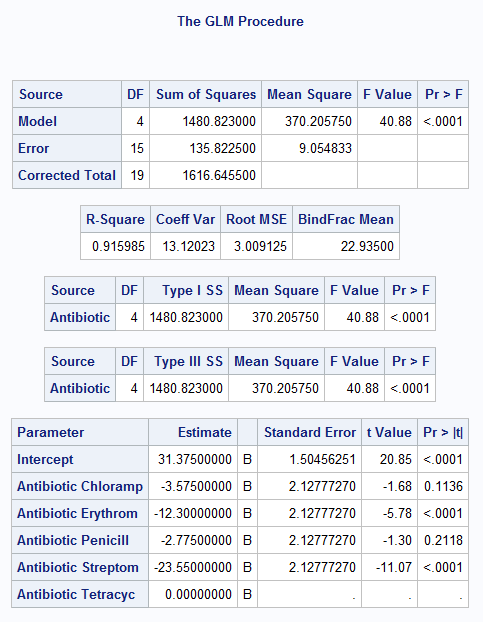
\includegraphics[scale=0.7]{BindFracGLM}\\
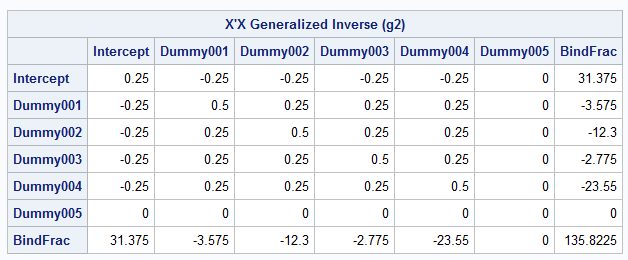
\includegraphics[scale=0.7]{BindFracGLMInverse}\\
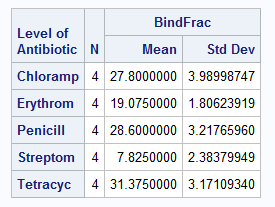
\includegraphics[scale=0.7]{BindFracMeans}
\end{flushleft}

\newpage

Estimates of the $\beta$'s still found by 
\[\hat{\boldsymbol{\beta}}= (\textbf{X}'\textbf{X})^{-1}\textbf{X}'\textbf{Y} = \left(\begin{array}{r} 31.375 \\ -3.575 \\ -12.300 \\
-2.775 \\ -23.550 \end{array} \right)
\]
~\\~\\

Estimates for the five treatment means obtained by using combinations from the $\hat{\boldsymbol{\beta}}$ vector 
$$\mu(x_1,x_2,x_3,x_4)=\beta_0 + \beta_1 x_1 + \beta_2 x_2 + \beta_3 x_3 + \beta_4 x_4$$
$$\mbox{Trt 1 estimate} = \hat\mu(1,0,0,0) = ~~~~~~~~~~~~~~~~~~~~~~~~~~~~~~~~~~~~~~~~~~~~~~~~~~~~~~~~~~~~~~~~~~~~~~~~~$$~\\
%\textcolor{red}{\hat\beta_0 + \hat\beta_1 =  27.800 $$}
$$\mbox{Trt 2 estimate} = \hat\mu(0,1,0,0) = ~~~~~~~~~~~~~~~~~~~~~~~~~~~~~~~~~~~~~~~~~~~~~~~~~~~~~~~~~~~~~~~~~~~~~~~~~$$~\\
%\textcolor{red}{\hat\beta_0 + \hat\beta_2 =  19.075 $$}
$$\mbox{Trt 3 estimate} = \hat\mu(0,0,1,0) = ~~~~~~~~~~~~~~~~~~~~~~~~~~~~~~~~~~~~~~~~~~~~~~~~~~~~~~~~~~~~~~~~~~~~~~~~~$$~\\
%\textcolor{red}{\hat\beta_0 + \hat\beta_3 =  28.600$$}
$$\mbox{Trt 4 estimate} = \hat\mu(0,0,0,1) = ~~~~~~~~~~~~~~~~~~~~~~~~~~~~~~~~~~~~~~~~~~~~~~~~~~~~~~~~~~~~~~~~~~~~~~~~~$$~\\
%\textcolor{red}{\hat\beta_0 + \hat\beta_4 =  ~7.825$$}
$$\mbox{Trt 5 estimate} = \hat\mu(0,0,0,0) = ~~~~~~~~~~~~~~~~~~~~~~~~~~~~~~~~~~~~~~~~~~~~~~~~~~~~~~~~~~~~~~~~~~~~~~~~~$$~\\
%\textcolor{red}{\hat\beta_0~~~~~~~ =  31.375$$}
~\\~\\~\\

For standard errors of the $\hat{\beta}$'s we still have our variance-covariance matrix $\hat{\boldsymbol{\Sigma}}=MS(E)(\textbf{X}^{T}\textbf{X})^{-1}$
\[ 
\hat{\boldsymbol{\Sigma}} = MS(E) (\textbf{X}'\textbf{X})^{-1} = \left(\begin{array}{rrrrr} 
2.264   & -2.264      & -2.264      & -2.264      & -2.264 \\
      & 4.527       & 2.264      & 2.264       & 2.264 \\
      &           & 4.527       & 2.264       & 2.264 \\
      &           &           & 4.527      & 2.264 \\
      &           &           &           & 4.527 \\
\end{array} \right)
\]

Note the pattern, what is the reason for it?\\~\\~\\~\\~\\
%\textcolor{red}{\\~\\The intercept represents a treatment mean, whereas all the other $\beta$'s represent differences between treatment means.}\\~\\

\newpage

To get SE's of our treatment mean estimates we can use vectors:  Let $\textbf{a},\textbf{b},\textbf{c},\textbf{d}$ be defined by 
$$\textbf{a}^{T}=(1,1,0,0,0), \textbf{b}^{T}=(1,0,1,0,0), \textbf{c}^{T}=(1,0,0,1,0), \textbf{d}^{T}=(1,0,0,0,1), \textbf{f}^{T}=(1,0,0,0,0).$$
Then
\[
\begin{array}{lclcl}
\hat\mu(1,0,0,0) & = & \hat\beta_0  + \hat\beta_1 & = & \textbf{a}^{T}\hat\beta \\
\hat\mu(0,1,0,0) & = & \hat\beta_0  + \hat\beta_2 & = & \textbf{b}^{T}\hat\beta \\
\hat\mu(0,0,1,0) & = & \hat\beta_0  + \hat\beta_3 & = & \textbf{c}^{T}\hat\beta \\
\hat\mu(0,0,0,1) & = & \hat\beta_0  + \hat\beta_4 & = & \textbf{d}^{T}\hat\beta \\
\hat\mu(0,0,0,0) & = & \hat\beta_0  & = & \hat\beta_0 
\end{array}
\]~\\
and for a balanced design the variances are all the same and are given by
$$\textbf{a}^{T} \hat{\boldsymbol{\Sigma}} \textbf{a} = \textbf{b}^{T} \hat{\boldsymbol{\Sigma}} \textbf{b} = \textbf{c}^{T} \hat{\boldsymbol{\Sigma}} \textbf{c} = \textbf{d}^{T} \hat{\boldsymbol{\Sigma}} \textbf{d} = \textbf{f}^{T}\hat{\boldsymbol{\Sigma}}\textbf{f}= \widehat{\Var}(\hat\beta_0) = \widehat{\Var}(\hat\beta_0 + \hat\beta_j) = 2.264$$
Note: 
$$\widehat{\Var}(\hat\beta_0 + \hat\beta_j) =\widehat{\Var}(\hat\beta_0)+\widehat{\Var}(\hat\beta_j)+2\widehat{Cov}(\hat\beta_0,\hat\beta_j) = 2.264+4.527+2*(-2.264)=2.263~~~(rounding)$$
so the estimated SE for any sample treatment mean is \\~\\~\\~\\~\\~\\~\\
%\textcolor{red}{$$\sqrt{2.264}=1.505$$}\\~\\

Recall from one-way ANOVA that 
$$\widehat{SE}(\bar{Y}_{i\bullet}) = \sqrt{\frac{MS(E)}{n}} = \sqrt{\frac{9.055}{4}} = \sqrt{2.264} = 1.505$$
and that for differences between treatment means 
$$\widehat{SE}(\bar{Y}_{i\bullet}-\bar{Y}_{j\bullet})=\sqrt{\frac{2MS(E)}{n}}=\sqrt{4.528} = 2.128$$
which is $\sqrt{4.527}$!
~\\~\\

\textbf{Using dummy variables, we can now easily include both quantitative and categorical explanatory variables at the same time!}

\newpage

\Large\textbf{A general linear model for 5k times of men AND women:}\large\\
Using $x_1$=Age, we fit a quadratic model $\mu(x_1) = \beta_0 + \beta_1 x_1 + \beta_2 x_1^2$ to predict the mean pace for runners.  Consider modeling gender (a categorical variable with 2 levels, implying we need 2-1=1 dummy variable) as well.\\

Let $x_3$ be defined by  
\[
x_3 = 
\begin{cases} 
1 & \text{female} \\ 0 & \text{male} 
\end{cases}
\]~\\

Some candidate models:
\begin{enumerate}
\item The `null' model:
$$\mu(x_1,x_3) = \beta_0$$~\\~\\
%\textcolor{red}{Just use the overall mean pace to predict for any age and any gender.}
\item The One-Way ANOVA model in GLM form:
$$\mu(x_1,x_3) = \beta_0 + \beta_3 x_3$$~\\~\\
%\textcolor{red}{A model that uses the mean pace for men to predict for all men and the mean pace for women to predict for all women.}
\item The SLR model using Age:
$$\mu(x_1,x_3) = \beta_0 + \beta_1 x_1$$~\\~\\
%\textcolor{red}{Pace has a linear relationship with age, same relationship for both men and women.}
\item The GLM model using Age and Gender:
$$\mu(x_1,x_3) = \beta_0 + \beta_1 x_1 + \beta_3 x_3$$~\\~\\
%\textcolor{red}{Pace has a linear relationship with age, different intercept for men and women.}
\item The GLM model using Age, Gender, and their Interaction:
$$\mu(x_1,x_3) = \beta_0 + \beta_1 x_1 + \beta_3 x_3+\beta_4x_1x_3$$~\\~\\
%\textcolor{red}{Pace has a linear relationship with age, different intercept and slope for men and women.}
\item The MLR model quadratic in Age:
$$\mu(x_1,x_3) = \beta_0 + \beta_1 x_1+ \beta_2 x_1^2 $$~\\~\\
%\textcolor{red}{Pace has a quadratic relationship with age, same parabola for both men and women.}
\item The GLM model quadratic in Age with a gender main effect:
$$\mu(x_1,x_3) = \beta_0 + \beta_1 x_1+ \beta_2 x_1^2+ \beta_3 x_3$$~\\~\\~\\~\\~\\~\\~\\~\\~\\
%\textcolor{red}{Pace has a quadratic relationship with age, different intercepts for the men and women parabolas.\\
%This model has intercept $\beta_0$ for males ($x_3=0$) and intercept $\beta_0+\beta_3$ for females ($x_3=1$).
%$$\mbox{Equation for males: } \beta_0+\beta_1x_1+\beta_2x_1^2$$
%$$\mbox{Equation for females: } (\beta_0+\beta_3)+\beta_1x_1+\beta_2x_1^2$$}
\item A GLM model quadratic in Age with all gender interactions:
$$\mu(x_1,x_3) = \beta_0 + \beta_1 x_1+ \beta_2 x_1^2+ \beta_3 x_3 + \beta_4 x_1x_3 + \beta_5x_1^2x_3 $$
%\textcolor{red}{Pace has a quadratic relationship with age, different intercepts and different shapes of the parabolas.\\
%Intercepts as in the previous model.  `Linear' term for males is $\beta_1$ and is $\beta_1+\beta_4$ for females.  `Quadratic' term for males is $\beta_2$ and is $\beta_2+\beta_5$ for females. 
%$$\mbox{Equation for males: } \beta_0+\beta_1x_1+\beta_2x_1^2$$
%$$\mbox{Equation for females: } (\beta_0+\beta_3)+(\beta_1+\beta_4)x_1+(\beta_2+\beta_5)x_1^2$$}
\end{enumerate}

\newpage

We can fit these models in proc glm using the following code: (Note: each model must be done in a separate proc glm statement)
\begin{small}
\begin{verbatim}
*Note, you would need to run a different proc glm for each model;
proc glm;  
title 'Model 2'; class sex; model pace=sex/solution clparm;
title 'Model 3';            model pace=age/solution clparm;
title 'Model 4'; class sex; model pace=age sex/solution clparm;
title 'Model 5'; class sex; model pace=age sex age*sex/solution clparm;
title 'Model 6';            model pace=age age*age/solution clparm;
title 'Model 7'; class sex; model pace=age age*age sex/solution clparm;
title 'Model 8'; class sex; model pace=age age*age sex sex*age sex*age*age/solution clparm;
run;
\end{verbatim}
\end{small}

\begin{flushleft}
\includegraphics[scale=0.8,page=2,trim=5mm 85mm 5mm 5mm]{ResRunGLM.pdf}
\includegraphics[scale=0.7,trim= 5mm 100mm 5mm 5mm,page=3]{ResRunGLM.pdf}
\includegraphics[scale=0.8,page=5,trim=5mm 100mm 5mm 15mm]{ResRunGLM.pdf}
\includegraphics[scale=0.8,trim= 5mm 150mm 5mm 5mm,page=6]{ResRunGLM.pdf}
\includegraphics[scale=0.8,page=8,trim=5mm 85mm 5mm 5mm]{ResRunGLM.pdf}
\includegraphics[scale=0.8,trim= 5mm 150mm 5mm 5mm,page=9]{ResRunGLM.pdf}
\includegraphics[scale=0.8,page=11,trim=5mm 85mm 5mm 5mm]{ResRunGLM.pdf}
\includegraphics[scale=0.8,trim= 5mm 150mm 5mm 5mm,page=12]{ResRunGLM.pdf}
\includegraphics[scale=0.8,page=14,trim=5mm 85mm 5mm 5mm]{ResRunGLM.pdf}
\includegraphics[scale=0.8,trim= 5mm 5mm 5mm 5mm,page=15]{ResRunGLM.pdf}
\includegraphics[scale=0.8,trim= 5mm 5mm 5mm 5mm,page=17]{ResRunGLM.pdf}
\includegraphics[scale=0.8,trim= 5mm 5mm 5mm 5mm,page=18]{ResRunGLM.pdf}
\includegraphics[scale=0.8,trim= 5mm 5mm 5mm 5mm,page=20]{ResRunGLM.pdf}
\includegraphics[scale=0.8,trim= 5mm 5mm 5mm 5mm,page=21]{ResRunGLM.pdf}
\end{flushleft}

For model 7 the fitted model is
\[
\hat{\mu}(x_1,x_3)=\begin{cases}  
\hat{\beta}_0 + \hat{\beta}_1 x_1 + \hat{\beta}_2 x_1^2 + \hat{\beta}_3 (0)
& \text{ for men} \\
\fbox{$=10.18 - 0.17 x +0.0028 x^2$} & \\
\hat{\beta}_0 + \hat{\beta}_3+\hat{\beta}_1 x_1 + \hat{\beta}_2 x_1^2
& \text{ for women} \\
\fbox{$=(10.18 + 2.20) - 0.17 x_1 +0.0028 x_1^2$} & \\
\end{cases}
\]
For model 8 the fitted model is
\[
\hat{\mu}(x_1,x_3)=\begin{cases} 
\hat{\beta}_0 + \hat{\beta}_1 x_1 + \hat{\beta}_2 x_1^2 + \hat{\beta}_3 (0) + \hat{\beta}_4(0) + \hat{\beta}_5(0)
& \text{men} \\
\fbox{$10.61 - 0.20 x_1 +0.0032 x_1^2$} & \\
\hat{\beta}_0 + \hat{\beta}_1 x_1 + \hat{\beta}_2 x_1^2 + \hat{\beta}_3 (1) + \hat{\beta}_4 (x_1) + \hat{\beta}_5(x_1^2) & \text{women} \\ 
(\hat{\beta}_0 + \hat{\beta}_3) + (\hat{\beta}_1 + \hat{\beta}_4)x_1 + (\hat{\beta}_2 + \hat{\beta}_5)x_1^2 & \\
(10.61 + 1.26) + (-0.20 +0.07) x_1 + (0.0032 -0.0010) x_1^2  & \\
\fbox{$11.87 - 0.13 x_1 + 0.0022  x_1^2$}  & \\
\end{cases}
\]
Which model is ``better"?  What do we mean by ``better?"  Is there a test we can use to compare these models?\\~\\~\\~\\~\\
%\textcolor{red}{\\Yes!  F-test for nested models can be used (LOF test).}\\~\\

\textbf{Comparison of models 7 and 8:}\\
\begin{eqnarray*}
\text{reduced:  } \mu(x_1,x_3) &=& \beta_0 + \beta_1 x_1+ \beta_2 x_1^2+ \beta_3 x_3  \\
\text{full:  } \mu(x_1,x_3) &=& \beta_0 + \beta_1 x_1+ \beta_2 x_1^2+ \beta_3 x_3 + \beta_4 x_1x_3 + \beta_5 x_1^2 x_3
\end{eqnarray*}
Extra Regression sum of squares: 
%$$R(\beta_4,\beta_5|\beta_0,\beta_1,\beta_2) = SS[R]_f - SS[R]_r = 293.5 - 290.3 =3.2$$
%$$SS(R)_f - SS(R)_r = 293.5 - 290.3 =3.2$$
$$SS(R)_f - SS(R)_r = ~~~~~~~~~~~~~~~~~~~~~~~~~~~~~~~~~~~~~~~~~~~~~~~~~~~~~~~~~~~~~~~$$

The $F$-ratio 
%$$F=\frac{\left(SS(R)_f - SS(R)_r\right)/(p-q)}{MS(E)_f} = \frac{3.2/2}{3.21} = \frac{1.6}{3.21} = 0.5 $$
$$F=\frac{\left(SS(R)_f - SS(R)_r\right)/(p-q)}{MS(E)_f} = ~~~~~~~~~~~~~~~~~~~~~~~~~~~~~~~~~~~~~~~~~~~~~~~~~~~~~~~~~~~~~~~~~~~~~~~~~$$
The observed $F$-ratio is not significant for an F with $df=2,154$ $F_{0.05,2,154}=3.05$.\\~\\

As the age squared term and sex term are both significant using a type III test, the model quadratic in Age that has separate intercepts for males and females seems appropriate (model 7 seems good).

\newpage

\Large\textbf{Analysis of covariance, ANCOVA or ACOVA:}\large\\
Recall the three principles of experimental design:
\begin{itemize}
\item Randomization
\item Replication
\item Error Reducing Methods
\end{itemize}

One method of error reduction we looked at was blocking.  Here we split up the EUs and then randomize treatments to each block.  In this way, every treatment occurs in each block and the block effects cancel out.\\~\\
We are not always able to block, sometimes we don't have the value of the covariate until after the experiment is done.  A similar method that will account for these types of covariates is called Analysis of CoVariance (ANCOVA).\\~\\
Associations between covariates $z$ and the main response variable of interest $y$ can be used to reduce unexplained variation $\sigma^2$, allowing for clearer estimates of treatment effects.\\~\\

\textbf{An nutrition example:}\\
A nutrition scientist conducted an experiment to evaluate the effects of four vitamin supplements on the weight gain of laboratory animals.  The experiment was conducted in a completely randomized design with $N=20$ animals randomized to $a=4$ supplement groups, each with sample size $n\equiv 5$.  The response variable of interest is weight gain, but calorie intake $z$ was measured concomitantly as couldn't separate EUs by this at the beginning.  
~\\
\begin{center}
\begin{tabular}{|cc|cc|cc|cc|} \hline
Diet & $y$ & Diet & $y$ &Diet & $y$ &Diet & $y$ \\ \hline
1 & 48 & 2 & 65 & 3 & 79 & 4 & 59 \\
1 & 67 & 2 & 49 & 3 & 52 & 4 & 50 \\
1 & 78 & 2 & 37 & 3 & 63 & 4 & 59 \\
1 & 69 & 2 & 75 & 3 & 65 & 4 & 42 \\
1 & 53 & 2 & 63 & 3 & 67 & 4 & 34 \\ \hline
1 & $\bar{y}_{1\bullet}=63.0$ & 2 & $\bar{y}_{2\bullet}=57.4$  & 3 & $\bar{y}_{3\bullet}=65.2$  & 4 & $\bar{y}_{4\bullet}=48.8$ \\
1 & $s_1=12.3$ & 2 & $s_2=14.3$  & 3 & $s_3=9.7$  & 4 & $s_4=10.9$ \\ \hline
\end{tabular} 
\end{center}
~\\

Main question: Is there evidence of a vitamin supplement effect?
%\textcolor{red}{$H_0:$}

\newpage

\begin{center}
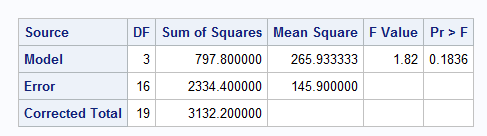
\includegraphics{DietsANOVA}
\end{center}
 
P-value $>$ 0.05, fail to reject $H_0$.  There is no evidence of a diet effect.\\~\\~\\

Calorie intake $z$ was measured concomitantly:
\begin{center}
\begin{tabular}{ccc|ccc|ccc|ccc}
Diet & $y$ & $z\ \ $ & Diet & $y$ & $z\ \ $ &Diet & $y$ & $z\ \ $ &Diet & $y$ & $z\ \ $ \\ \hline
1 & 48 & 350 & 2 & 65 & 400 & 3 & 79 & 510 & 4 & 59 & 530 \\
1 & 67 & 440 & 2 & 49 & 450 & 3 & 52 & 410 & 4 & 50 & 520 \\
1 & 78 & 440 & 2 & 37 & 370 & 3 & 63 & 470 & 4 & 59 & 520 \\
1 & 69 & 510 & 2 & 73 & 530 & 3 & 65 & 470 & 4 & 42 & 510 \\
1 & 53 & 470 & 2 & 63 & 420 & 3 & 67 & 480 & 4 & 34 & 430 \\ \hline
\end{tabular} 
\end{center}

Why might we want to incorporate the caloric intake?\\~\\~\\~\\~\\~\\~\\

How can we incorporate the caloric intake into the model?\\~\\~\\~\\~\\
%\textcolor{red}{\\A GLM can take into account both types of variables!  The method of ANCOVA can be used to reduce unexplained variation. \\
%$$ Y_i = \beta_0 + \beta_1 x_{i1} + \beta_2 x_{i2} + \beta_3 x_{i3} + \beta_z z_i + E_i \ \ \mbox{ for }i=1,\ldots,20$$
%where $x_{ij}$ is an indicator variable for subject $i$ receiving vitamin supplement $j$:
%$$ x_{ij}=\begin{cases} 1 & \text{subject $i$ receives supplement $j$} \\  
%0 & \text{else} \end{cases}$$
%and errors $E_i \iid N(0,\sigma^2)$.\\~\\
%Which Diet is being used as the baseline?\\
%Diet 4}\\~\\

\newpage

\textbf{ANCOVA analysis}:
\begin{small}
\begin{verbatim}
proc glm data=diets;      class diet;     model gain = diet caloric;    run;
\end{verbatim}
\end{small}

\begin{flushleft}
\includegraphics[page=2,scale=0.7,trim = 5mm 120mm 5mm 5mm]{DietsANCOVA}
\includegraphics[page=3,scale=0.5,trim = 5mm 150mm 5mm 5mm]{DietsANCOVA}
\end{flushleft}

\newpage

What type of test should we do if we want to test for a diet effect \textit{once caloric intake has been accounted for}? Type I or Type III?\\~\\~\\~\\

To test for a diet effect once caloric intake has been accounted for: 
$$H_0: \beta_1 = \beta_2 = \beta_3 =0$$
we compare 6.51 to an F distribution with 3 numerator and 15 denominator degrees of freedom.  (Note that this is a comparison of nested models!)\\~\\

Conclusion?\\  ~\\~\\~\\~\\~\\
%\textcolor{red}{\\As $p-value=0.0049<0.05$, reject $H_0$ in favor of $H_A$.  At the 5\% significance level, there is enough evidence to conclude that a diet effect exists once caloric intake has been accounted for.}\\~\\

What now?  We know there is a difference due to diet.  If we look at the sample means of the weight gains for the diets we can compare their effectiveness.  However, the weight gain is also affected by caloric intake...\\~\\

\newpage

\Large\textbf{LSMEANS - Least Squares Means or Adjusted Means}\large\\
\textbf{Estimation of Mean Weight Gains for Diets, Taking into Account Caloric Intake}\\

\textbf{Adjusted vs unadjusted means:}\\
The sample mean weight gains for the four diets and for the caloric intake for each diet group were
\begin{center}
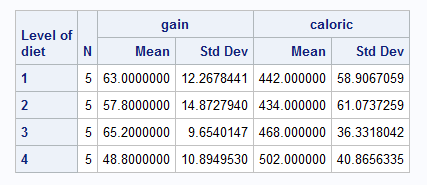
\includegraphics{DietsMeans}
\end{center}

The means for each diet are `unadjusted' means.  According to our analysis, caloric intake has a significant effect on weight gain.  However, each diet group had a different mean amount of caloric intake.  What does this imply?\\~\\~\\~\\~\\~\\~\\~\\~\\~\\~\\
%\textcolor{red}{\\~\\Some of the weight gain for diet 4 may be due to the fact that the caloric intake was much higher for this group.  Similarly, lack of weight gain in diet 2 may be due to low caloric intake}  \\~\\

Unadjusted means do not make any adjustment for the facts that 
\begin{enumerate}
\item caloric intake may vary by diet (presumably by chance, not because of diet)
\item weight gain depends on caloric intake
\end{enumerate}

\newpage

\textbf{Adjusted means} or \textbf{lsmeans} (least squares means) will estimate mean weight gains at a common value of our caloric intake (our covariate $z$).  The value often used for comparison is $\bar{z}$, the sample mean of the covariate.\\~\\

Here, $\bar{z}= (442+434+468+502)/4 = 461.5$.  The adjusted means are then just (the sub $a$ is to differentiate unadjusted means and adjusted means)
\begin{eqnarray*}
\bar{y}_{1,a} & = & \hat\beta_0 + \hat\beta_1 + \hat\beta_z (461.5) \\
\bar{y}_{2,a} & = & \hat\beta_0 + \hat\beta_2 + \hat\beta_z (461.5) \\
\bar{y}_{3,a} & = & \hat\beta_0 + \hat\beta_3 + \hat\beta_z (461.5) \\
\bar{y}_{4,a} & = & \hat\beta_0 + \hat\beta_z (461.5)
\end{eqnarray*} 

To get SAS to report the estimated regression parameter vector $\hat{\boldsymbol{\beta}}$, use the {\tt solution} option in the model statement.  The default parametrization is the one we've adopted here where $\beta_0$ is the mean of the last level of the classification treatment factor:

\begin{center}
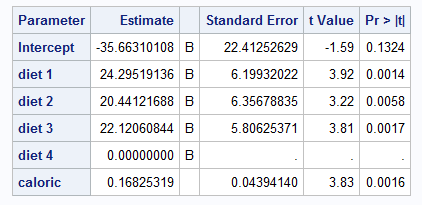
\includegraphics{DietsEstimates}
\end{center}

Substitution of $\hat{\boldsymbol{\beta}}$ into the expressions for adjusted means yields
\begin{eqnarray*}
\bar{y}_{1,a} & = & -35.7 + 24.3 + 0.17 (461.5) = 66.3\\
\bar{y}_{2,a} & = & -35.7 + 20.4 + 0.17 (461.5) = 62.4 \\
\bar{y}_{3,a} & = & -35.7 + 22.1 + 0.17 (461.5) = 64.1 \\
\bar{y}_{4,a} & = & -35.7 + + 0.17 (461.5) = 42.0 
\end{eqnarray*} 

These means are better for comparisons between diets as the effect of caloric intake (which affects weight gain) is constant across all the diets.  Thus, we are removing its effect.\\~\\

\newpage
\Large\textbf{Inference for Lsmeans}\large\\
We have our point estimate, $\bar{y}_{i,a}$.\\~\\
Now we need to know the \textbf{standard errors of }$\bar{Y}_{i,a}$\\~\\

Consider $\bar{Y}_{2,a}$.  What vector $c$ is needed so that $\textbf{c}^{T}\hat{\boldsymbol{\beta}} = \bar{Y}_{2,a}$? \\~\\~\\~\\~\\~\\
%\textcolor{red}{$$\textbf{c}^{T}=(1~~0~~1~~0~~461.5)$$~\\}

What is the standard error of $\textbf{c}^{T}\hat{\boldsymbol{\beta}}$?\\
$$Var(\textbf{c}^{T}\hat{\boldsymbol{\beta}}) =\textbf{c}^{T}\hat{\boldsymbol{\Sigma}}\textbf{c} = 17.198$$~\\
This implies 
$$SE(\textbf{c}^{T}\hat{\boldsymbol{\beta}})=\sqrt{17.198}=4.147$$~\\

By the normality, we can now form a CI for the lsmean using the usual $Estimate~\pm~t~\hat{SE}(Estimate)$.\\~\\

Here a 95\% CI for the true diet 2 mean weight gain when caloric intake is 461.5 is
$$\bar{Y}_{2,a}\pm t_{20-4-1,0.05/2}\hat{SE}(\bar{Y}_{2,a}) = 62.4 \pm 2.131(4.147) = (53.56,71.24)$$\\~\\

We are 95\% confident that the true mean weight gain for diet 2 when caloric intake is 461.5 is between 53.56 and 71.24 grams.\\~\\

\newpage

\Large\textbf{Inference for Lsmeans in SAS}\large\\

\begin{small}
\begin{verbatim}
proc glm data=diets;
class diet;
model gain = diet caloric/solution inverse;
means diet;
lsmeans diet/stderr cl;
run;
\end{verbatim}
\end{small}

\begin{center}
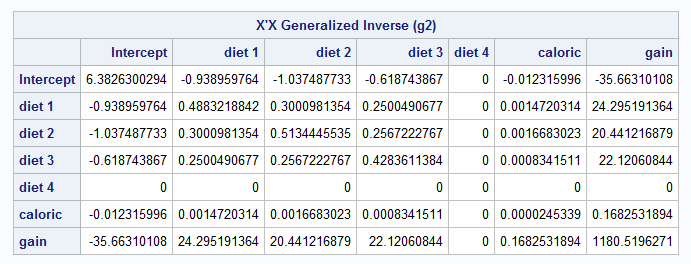
\includegraphics[scale=0.75]{DietsInverse}
\end{center}

The $(\textbf{X}^{T}\textbf{X})^{-1}$ matrix is found by removing the row/column with 0's and ignoring the row/column for the response.

\begin{flushleft}
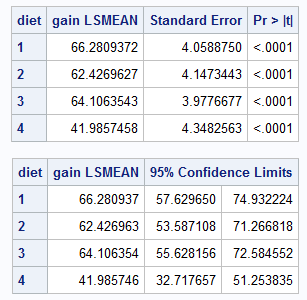
\includegraphics[scale=0.75]{DietsLSMeans}
\end{flushleft}

In One-Way Anova with a balanced design, all of the standard errors for the treatment means are equal.  Why do they differ here?

\newpage

\Large\textbf{Investigating Pairwise Differences of LSMeans}\large\\
We can now look at all pairwise differences of the lsmeans to see which levels differ significantly.  Inference for these differences of lsmeans can again be followed through using the MLR material.\\~\\

Consider testing the lsmean for group 1 vs that of group 4. \\~\\
Need to know \textbf{standard error of }$\bar{Y}_{1,a}-\bar{Y}_{4,a}$\\

Consider $\bar{Y}_{1,a}$.  From above we know we can find a vector $c_1$ so that $\textbf{c}^{T}_1\hat{\boldsymbol{\beta}} = \bar{Y}_{1,a}$ 
$$\textbf{c}_1^{T}=~~~~~~~~~~~~~~~~~~~~$$
Likewise, we can find $c_2$ so that $\textbf{c}^{T}_2\hat{\boldsymbol{\beta}} = \bar{Y}_{4,a}$ 
$$\textbf{c}_2^{T}=~~~~~~~~~~~~~~~~~~~~$$

Now we can find the estimate of 
$$\bar{y}_{1,a}-\bar{y}_{4,a} = \textbf{c}^{T}_1\hat{\boldsymbol{\beta}}-\textbf{c}^{T}_2\hat{\boldsymbol{\beta}}$$
We simply subtract the vectors elementwise and get
$$\bar{y}_{1,a}-\bar{y}_{4,a}= ~~~~~~~~~~~~~~~~~~~~~~~~~~~~~~~~~~~~~~~~~~~~~~~~~~~~~~~~$$~\\

Note: We could have plugged in any common value of the covariate, z, and it would cancel out!\\~\\

What is the standard error of $\textbf{c}^{T}_3\hat{\boldsymbol{\beta}}$?\\~\\~\\~\\
%$$Var(\textbf{c}^{T}_3\hat{\boldsymbol{\beta}}) =\textbf{c}^{T}_3\hat{\boldsymbol{\Sigma}}\textbf{c}_3 = 38.4313$$
%$$\mbox{This implies } SE(\textbf{c}_3^{T}\hat{\boldsymbol{\beta}})=\sqrt{38.4313}=6.1993$$
We can now form a CI for this difference in lsmeans using the usual $Estimate~\pm~t~\hat{SE}(Estimate)$.\\~\\
Here a 95\% interval is: 
$$\bar{y}_{1,a}-\bar{y}_{4,a}\pm t_{20-4-1,0.05/2}\hat{SE}(\bar{y}_{1,a}-\bar{y}_{4,a}) =  24.295\pm 2.131(6.1993) = (11.084,37.506)$$\\~\\
As 0 is not in this interval, we are 95\% confident that the two treatment group means differ significantly if they have the same caloric intake.\\~\\

\newpage

\Large\textbf{Investigation of Pairwise Differences of LSMeans using SAS}\large
\begin{small}
\begin{verbatim}
proc glm data=diets;  class diet;
model gain = diet caloric/solution inverse;
lsmeans diet/adjust=tukey cl;  run;
\end{verbatim}
\end{small}

\begin{flushleft}
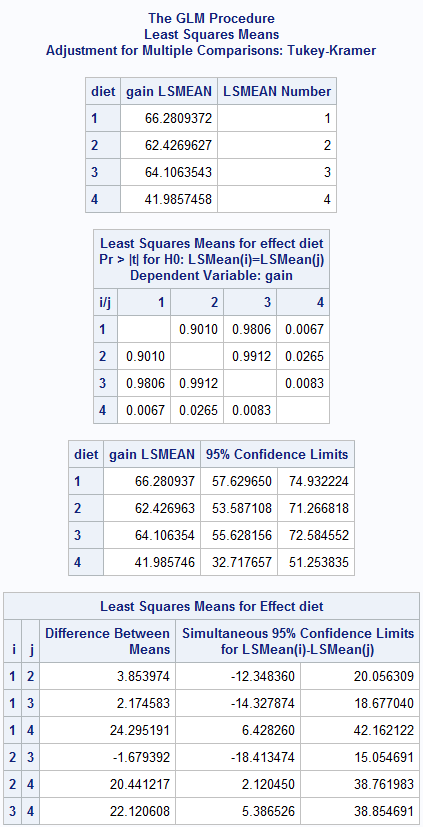
\includegraphics[scale=0.8]{DietsTukey}
\end{flushleft}

\newpage

\textbf{ANCOVA - What did we just do?  We used our covariate to reduce the unexplained variation in our response, allowing a clearer picture of our treatment differences. } \\~\\

\textbf{Huge assumptions of ANCOVA} - We assume the treatment \textit{does not} affect the covariate.  In this example, we assume the diets are not causing the animals to have different caloric intake (i.e. do not cause them to eat more or less). (We also need to do our usual assumption checking.)\\~\\
 We can inspect this assumption.  Let our covariate be our response and conduct an ANOVA using the diets as our treatments.  The global p-value will test if the caloric intake means differ significantly for each diet.  We hope to see no significance here!

\begin{small}
\begin{verbatim}
proc anova data=diets;
class diet;
model caloric = diet;
run;
\end{verbatim}
\end{small}

\begin{flushleft}
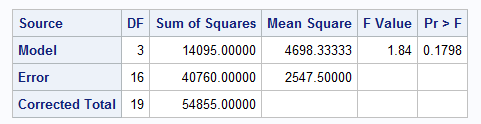
\includegraphics{DietsCaloricANOVA}
\end{flushleft}

No evidence that treatment affects covariate.\\~\\




